\documentclass[12pt, titlepage]{article}

\usepackage{fullpage}
\usepackage[round]{natbib}
\usepackage{multirow}
\usepackage{booktabs}
\usepackage{tabularx}
\usepackage{graphicx}
\usepackage{float}
\usepackage{hyperref}
\hypersetup{
    colorlinks,
    citecolor=black,
    filecolor=black,
    linkcolor=red,
    urlcolor=blue
}
\usepackage[round]{natbib}

\newcounter{acnum}
\newcommand{\actheacnum}{AC\theacnum}
\newcommand{\acref}[1]{AC\ref{#1}}

\newcounter{ucnum}
\newcommand{\uctheucnum}{UC\theucnum}
\newcommand{\uref}[1]{UC\ref{#1}}

\newcounter{mnum}
\newcommand{\mthemnum}{M\themnum}
\newcommand{\mref}[1]{M\ref{#1}}

\title{SE 3XA3: Software Requirements Specification\\BigTwo}

\author{Team 06, Team Name: Aplus^3
		\\ Senni Tan, tans28
		\\ Manyi Cheng, chengm33
		\\ Jiaxin Tang, tangj63
}

\date{\today}

%\input{../../Comments}

\begin{document}

\maketitle

\pagenumbering{roman}
\tableofcontents
\listoftables
\listoffigures

\begin{table}[bp]
\caption{\bf Revision History}
\begin{tabularx}{\textwidth}{p{3cm}p{2cm}X}
\toprule {\bf Date} & {\bf Version} & {\bf Notes}\\
\midrule
Mar 13, 2021 & 0.0 & Initial draft\\
\textcolor{red}{Apr 10, 2021} & \textcolor{red}{1.0} & \textcolor{red}{Revision 1.0}\\
\bottomrule
\end{tabularx}
\end{table}

\newpage

\pagenumbering{arabic}

\section{Introduction}
\subsection{Overview}
The BigTwo project is a re-implementation of an open-source LAN server game that was originally found on GitHub. The original project was implemented in Java, and our re-implementation will be in JavaScript and CSS. Our project, the BigTwo game, is a web-based card game that allows the user to play alone in a web browser with mouse clicking on the computer screen to interact with the game.

\subsection{Purpose}
This Module Guide document will provide the information about the structure in our module design, for the stakeholders including professor Bokhari, TAs in course SE3XA3, project developers to have a document to trace along wtih the project development, and also to understand the structure of the module design for this project.

\subsection{Context}
Decomposing a system into modules is a commonly accepted approach to developing
software.  A module is a work assignment for a programmer or programming
team~\citep{ParnasEtAl1984}.  We advocate a decomposition
based on the principle of information hiding~\citep{Parnas1972a}.  This
principle supports design for change, because the ``secrets'' that each module
hides represent likely future changes.  Design for change is valuable in SC,
where modifications are frequent, especially during initial development as the
solution space is explored.  

\subsection{Design Principles}
Our design follows the rules layed out by \citet{ParnasEtAl1984}, as follows:
\begin{itemize}
\item System details that are likely to change independently should be the
  secrets of separate modules.
\item Each data structure is used in only one module.
\item Any other program that requires information stored in a module's data
  structures must obtain it by calling access programs belonging to that module.
\end{itemize}

\subsection{Design Requirements}
After completing the first stage of the design, the Software Requirements
Specification (SRS), the Module Guide (MG) is developed~\citep{ParnasEtAl1984}. The MG
specifies the modular structure of the system and is intended to allow both
designers and maintainers to easily identify the parts of the software.  The
potential readers of this document are as follows:

\begin{itemize}
\item New project members: This document can be a guide for a new project member
  to easily understand the overall structure and quickly find the
  relevant modules they are searching for.
\item Maintainers: The hierarchical structure of the module guide improves the
  maintainers' understanding when they need to make changes to the system. It is
  important for a maintainer to update the relevant sections of the document
  after changes have been made.
\item Designers: Once the module guide has been written, it can be used to
  check for consistency, feasibility and flexibility. Designers can verify the
  system in various ways, such as consistency among modules, feasibility of the
  decomposition, and flexibility of the design.
\item Professor and TAs in course SE3XA3: This document can be a reference for the professor and TAs in course SE3XA3 to trace our process in project development, and to understand the overall structure of our module design.
\end{itemize}

\subsection{Document Structure}
The rest of the document is organized as follows. 
\begin{itemize}
    \item Section \ref{SecChange} lists the anticipated and unlikely changes of the software requirements.
    \item Section \ref{SecMH} summarizes the module decomposition that was constructed according to the likely changes.
    \item Section \ref{SecConnection} specifies the connections between the software requirements and the modules.
    \item Section \ref{SecMD} gives a detailed description of the modules.
    \item Section \ref{SecTM} includes two traceability matrices. One checks the completeness of the design against the requirements provided in the SRS. The other shows the relation between anticipated changes and the modules.
    \item Section \ref{SecUse} describes the use relation between modules.
\end{itemize}


\section{Anticipated and Unlikely Changes} \label{SecChange}

This section lists possible changes to the system. According to the likeliness
of the change, the possible changes are classified into two
categories. Anticipated changes are listed in Section \ref{SecAchange}, and
unlikely changes are listed in Section \ref{SecUchange}.

\subsection{Anticipated Changes} \label{SecAchange}

Anticipated changes are the source of the information that is to be hidden
inside the modules. Ideally, changing one of the anticipated changes will only
require changing the one module that hides the associated decision. The approach
adapted here is called design for change.

\begin{description}
\item[\refstepcounter{acnum} \actheacnum \label{acInterface}:] The graphical user interface used to display the various elements of the game, and retrieve user input.
\item[\refstepcounter{acnum} \actheacnum \label{acInput}:] The format of the
input data.
\item[\refstepcounter{acnum} \actheacnum \label{acOutput}:] The format of the
output data.
\item[\refstepcounter{acnum} \actheacnum \label{acLibrary}:] The actual implementation of the components.
\item[\refstepcounter{acnum} \actheacnum \label{acImplementation}:] The implementation of the classes and objects for Cards, PlayField, Players and Scene.

\end{description}

\subsection{Unlikely Changes} \label{SecUchange}

The module design should be as general as possible. However, a general system is
more complex. Sometimes this complexity is not necessary. Fixing some design
decisions at the system architecture stage can simplify the software design. If
these decision should later need to be changed, then many parts of the design
will potentially need to be modified. Hence, it is not intended that these
decisions will be changed.

\begin{description}
\item[\refstepcounter{ucnum} \uctheucnum \label{ucIO}:] Input/Output devices
  (Input: Mouse clicks, Output: Screen). The game will take the input from the user mouse clicking interaction with the game, and output the result to the screen.
\item[\refstepcounter{ucnum} \uctheucnum \label{ucPurpose}:] The purpose of the game to allow the user to play the BigTwo card game.
\item[\refstepcounter{ucnum} \uctheucnum \label{ucUser}:] The amount of user player: out game only allow single-player mode so only one user player is allowed in a game.
\item[\refstepcounter{ucnum} \uctheucnum \label{ucRule}:] The game rule of BigTwo: there are many versions on BigTwo game, we will take the Cantonese version of rules in our project.
\end{description}

\section{Module Hierarchy} \label{SecMH}

This section provides an overview of the module design. Modules are summarized
in a hierarchy decomposed by secrets in Table \ref{TblMH}. The modules listed
below, which are leaves in the hierarchy tree, are the modules that will
actually be implemented.

\begin{description}
\item [\refstepcounter{mnum} \mthemnum \label{mHH}:] Hardware-Hiding Module: Hardware-Hiding Module
\item [\refstepcounter{mnum} \mthemnum \label{mHH}:] Behaviour-Hiding Module: \textcolor{red}{App} Module
\item [\refstepcounter{mnum} \mthemnum \label{mHH}:] Behaviour-Hiding Module:  Card Module
\item [\refstepcounter{mnum} \mthemnum \label{mHH}:]
Behaviour-Hiding Module:  Player Module
\item [\refstepcounter{mnum} \mthemnum \label{mHH}:] Behaviour-Hiding Module:  PlayerBot Module
\item [\refstepcounter{mnum} \mthemnum \label{mHH}:] \textcolor{red}{ Software Decision Module:}  Rules Module
\item [\refstepcounter{mnum} \mthemnum \label{mHH}:] Behaviour-Hiding Module: Game Module
\item [\refstepcounter{mnum} \mthemnum \label{mHH}:] Behaviour-Hiding Module:  GameplayField Module

\end{description}


\begin{table}[h!]
\centering
\begin{tabular}{p{0.3\textwidth} p{0.6\textwidth}}
\toprule
\textbf{Level 1} & \textbf{Level 2}\\
\midrule

\multirow{1}{0.3\textwidth}{Hardware-Hiding Module} & Hardware-Hiding Module \\
\midrule

\multirow{7}{0.3\textwidth}{Behaviour-Hiding Module} & \textcolor{red}{App} Module\\
& Card Module\\
& Player Module\\
& PlayerBot Module\\
& Game Module\\
& GameplayField Module\\
\midrule

\multirow{1}{0.3\textwidth}{Software Decision Module}
& \textcolor{red}{Rules Module}\\
\bottomrule

\end{tabular}
\caption{Module Hierarchy}
\label{TblMH}
\end{table}

\section{Connection Between Requirements and Design} \label{SecConnection}

The design of the system is intended to satisfy the requirements developed in
the SRS. In this stage, the system is decomposed into modules. The connection
between requirements and modules is listed in Table \ref{TblRT}. The \textcolor{red}{App} module will render the game and other objects in a browser. The Game module will connect all methods together and will be the only way the program is executed. The functional requirements will be satisfied throughout all modules. The Player Module will fulfill the Usability requirement as it is responsible for interaction between user and server. The Rules module is responsible for functional requirements related to BigTwo game rules. 

\noindent The non-functional requirements will be satisfied throughout all modules.
Look and feel will requirements will be implemented in the GameplayField and Game module. The game will be easy to access because the game will be deployed using the server. Performance requirements are key to the program and will be fulfilled throughout all modules, ensuring that each part of the game fulfills corresponding requirements. Cultural, Political, Health, and safety requirements will be implemented by not using any external images that may offend the user, and by reducing the use of blue color and promoting warm colors.

\section{Module Decomposition} \label{SecMD}

The following modules are decomposed according to the principle of ``information hiding'' proposed by \citet{ParnasEtAl1984}, which are broken down into \emph{Secret}, \emph{Service}, and \emph{Implemented By}. \emph{Secret}is a brief description of the design decision hidden by the module. \emph{Service} specifies what the module will do with details. \emph{Implemented By} indicates how the module is implemented. 

\subsection{Hardware Hiding Modules}

\begin{description}
\item[Secrets:]The implementation of the virtual machine.
\item[Services:]Serves as the interface between the software and the hardware, which allows the system to communicate with the software through input and output devices.  
\item[Implemented By:] Operating System
\end{description}

\subsection{Behaviour-Hiding Module}

\begin{description}
\item[Secrets:] Required behaviours
\item[Services:] Describes the virtual behaviour of the application according to software requirements specified in the software requirements specification(SRS). This module serves as an interpreter between the Hardware Hiding Module and the Software Decision Module to ensure the application behaves as expected.
\item[Implemented By:] N/A
\end{description}

\subsubsection{\textcolor{red}{App} Module}

\begin{description}
\item[Secrets:] \textcolor{red}{App}
\item[Services:] Stores the App of the game.
\item[Implemented By:] \textcolor{red}{React.js}
\end{description}

\subsubsection{Card Module}

\begin{description}
\item[Secrets:] Card
\item[Services:] Generates and updates the cards of the game.
\item[Implemented By:] \textcolor{red}{React.js}
\end{description}

\subsubsection{Player Module}

\begin{description}
\item[Secrets:] Player Model
\item[Services:] Allows the user to select cards to play in the game.
\item[Implemented By:] \textcolor{red}{React.js}
\end{description}

\subsubsection{PlayerBot Module}

\begin{description}
\item[Secrets:] PlayerBot Model
\item[Services:] Serves as computer player to play with the user according to user inputs.
\item[Implemented By:] JavaScript Libraries
\end{description}

\subsubsection{Game Module}

\begin{description}
\item[Secrets:] Game
\item[Services:] Stores and updates the state of the game according to user inputs.
\item[Implemented By:] \textcolor{red}{React.js}
\end{description}

\subsubsection{GameplayField Module}

\begin{description}
\item[Secrets:] GameplayField
\item[Services:] Arranges players.
\item[Implemented By:] \textcolor{red}{React.js}
\end{description}

\subsection{Software Decision Module}

\begin{description}
\item[Secrets:] Data Structures
\item[Services:] Provides data structures to store information for the application.
\item[Implemented By:] N/A
\end{description}

\subsection{Be Module}
\subsubsection{Rules Module}

\begin{description}
\item[Secrets:] Rules
\item[Services:] Stores the rules of the game.
\item[Implemented By:] JavaScript Libraries
\end{description}

\section{Traceability Matrix} \label{SecTM}

This section shows three traceability matrices: between the modules and functional requirements, between the modules and non-functional requirements, and between the modules and the anticipated changes.

% the table should use mref, the requirements should be named, use something
% like fref
\begin{table}[H]
\centering
\begin{tabular}{p{0.2\textwidth} p{0.6\textwidth}}
\toprule
\textbf{Req.} & \textbf{Modules}\\
\midrule
FR1 & M3, M4, M6 \\
FR2 & M2\\
FR3 & M2, M7\\
FR4 & M2, M3, M7\\
FR5 & M2\\
FR6 & M2, M4, M7\\
FR7 & \textcolor{red}{M2, M4, M7}\\
FR8 & M8\\
FR9 & M7\\
FR10 & M2\\
FR11 & M2\\
FR12 & M7\\
FR13 & M6\\
FR14 & \textcolor{red}{M7, M8}\\
FR15 & \textcolor{red}{M7, M8}\\
FR16 & \textcolor{red}{M7, M8}\\
FR17 & \textcolor{red}{M7, M8}\\
\bottomrule
\end{tabular}
\caption{Trace Between Functional Requirements and Modules}
\label{TblRT}
\end{table}

\begin{table}[H]
\centering
\begin{tabular}{p{0.2\textwidth} p{0.6\textwidth}}
\toprule
\textbf{Req.} & \textbf{Modules}\\
\midrule
NF-L1 & M2\\
NF-L2 & M2\\
NF-L3 & M2\\
NF-L4 & M2\\
NF-L5 & M2, M3\\
NF-L6 & M2\\
NF-U1 & M4, M7\\
NF-U2 & M2, M4, M7\\
NF-U3 & M2\\
NF-U4 & M2\\
NF-A1 & M1\\
NF-P1 & M1\\
NF-P2 & \textcolor{red}{M6, M8}\\
NF-P3 & M1\\
NF-O1 & M1\\
NF-C1 & M2\\
NF-Le1 & M2\\
NF-C2 & M2, M7\\
NF-H1 & M2\\
\bottomrule
\end{tabular}
\caption{Trace Between Non-functional Requirements and Modules}
\label{TblRT}
\end{table}

\begin{table}[H]
\centering
\begin{tabular}{p{0.2\textwidth} p{0.6\textwidth}}
\toprule
\textbf{AC} & \textbf{Modules}\\
\midrule
AC1 & M1\\
AC2 & \textcolor{red}{M7}\\
AC3 & M1\\
AC4 & M1 \\
AC5 & M1\\
\bottomrule
\end{tabular}
\caption{Trace Between Anticipated Changes and Modules}
\label{TblACT}
\end{table}

\section{Use Hierarchy Between Modules} \label{SecUse}

\begin{figure}[H]
\centering
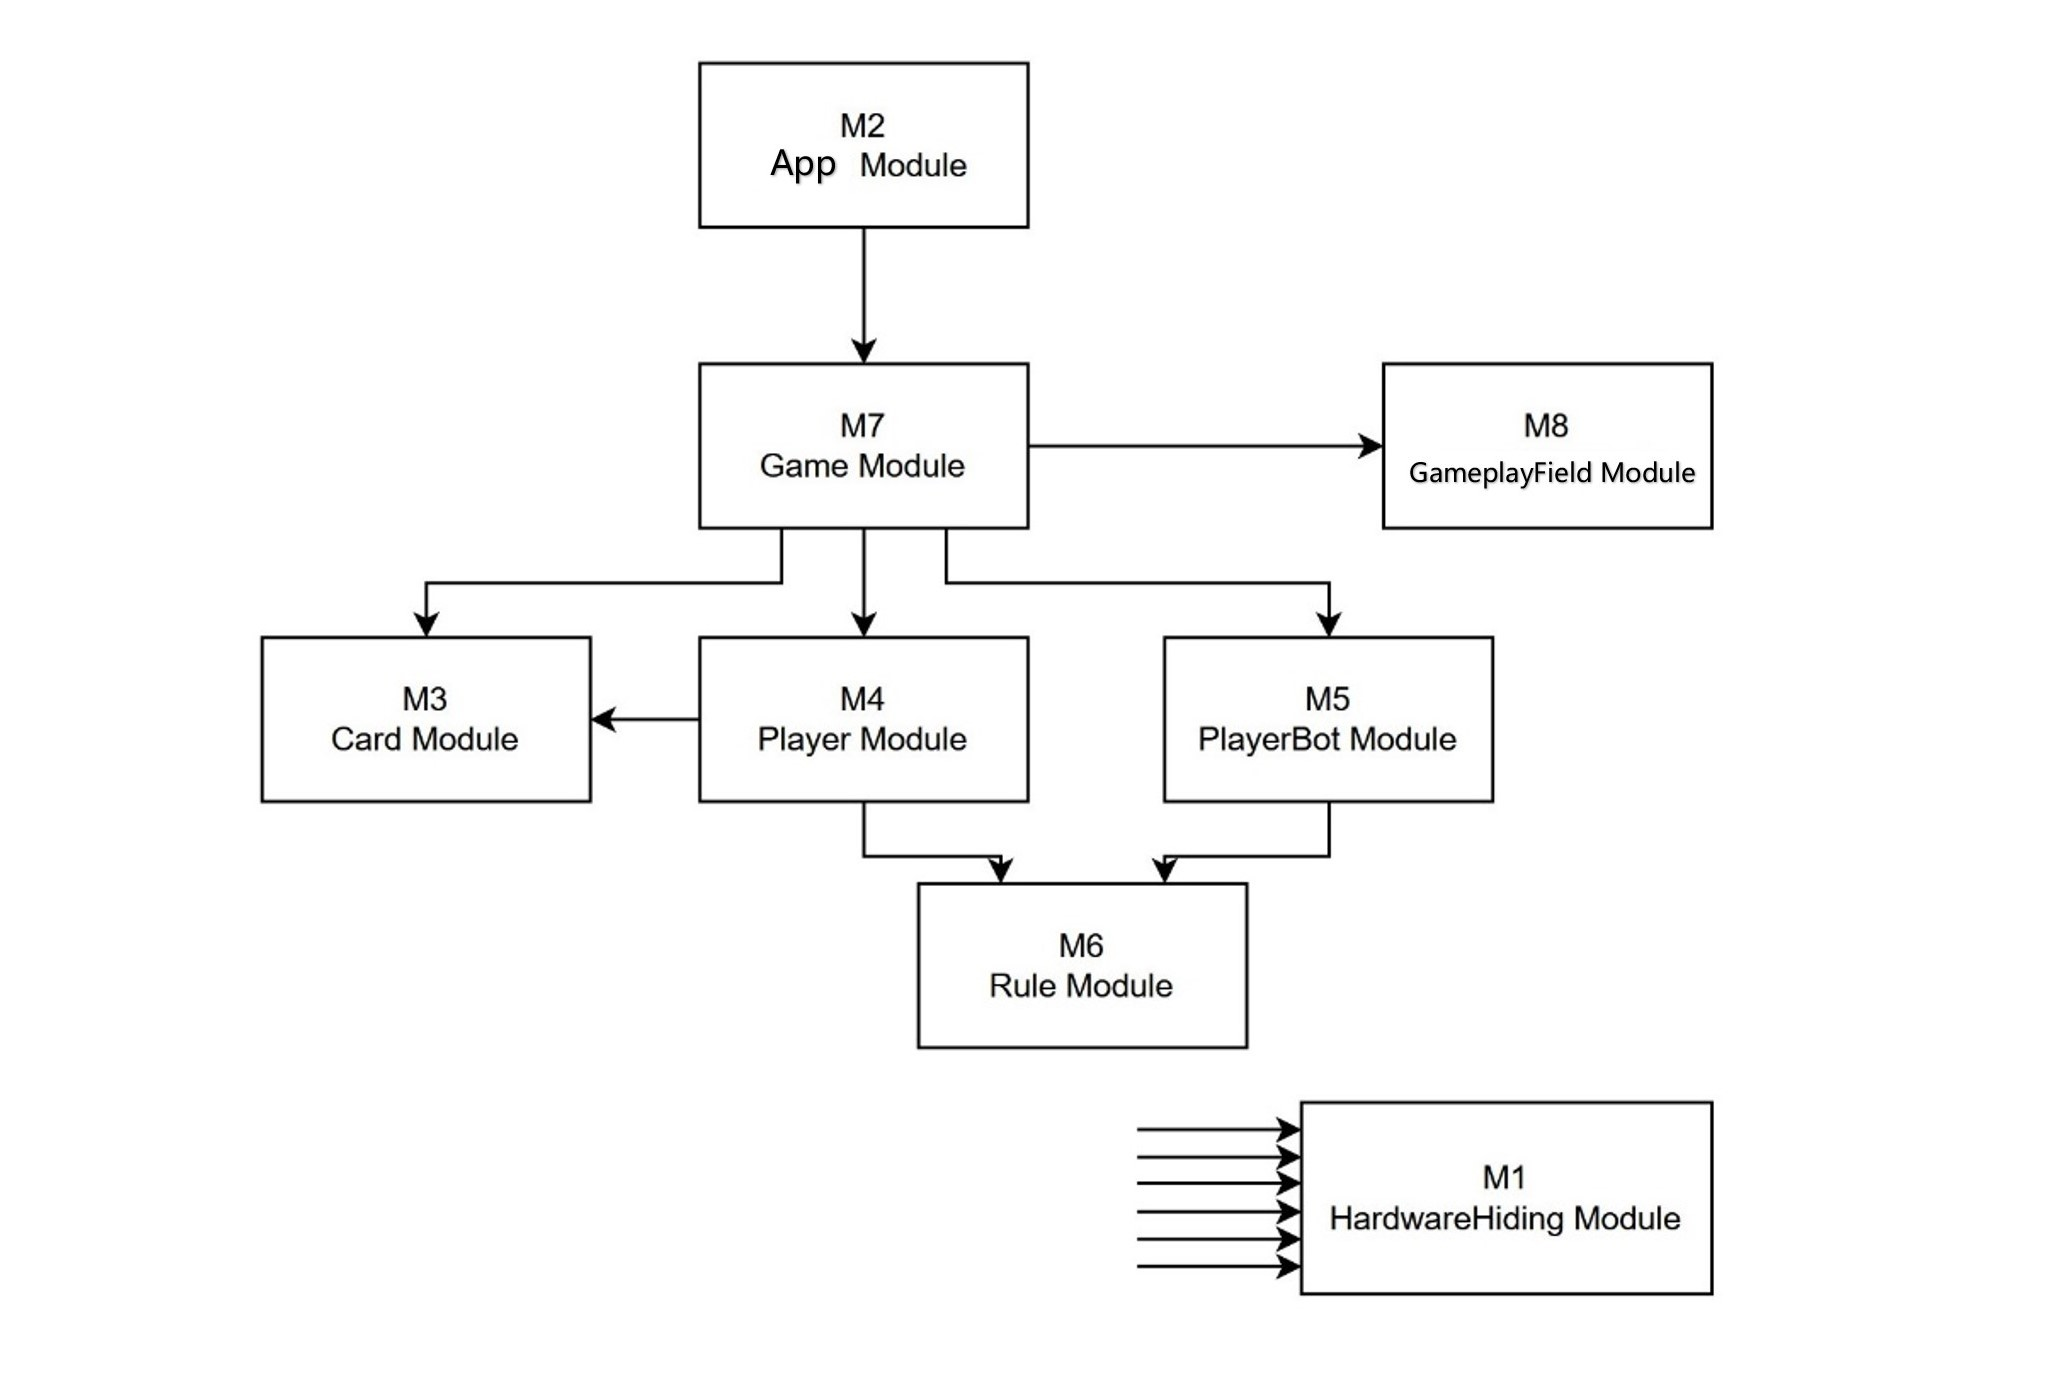
\includegraphics[width=1\textwidth]{UHD.jpg}
\caption{Use hierarchy among modules}
\label{FigUH}
\end{figure}
\newpage
%\section*{References}

\bibliographystyle {plainnat}
\bibliography {MG}

\end{document}